% LaTeX-Vorlage Medizintechnik Projektarbeit
% Alexander Ruppel
% veraendert von Eva Eibenberger 
% veraendert von Stephan Seitz

% %%%%%%%%%%%%%%%%%%%%%%%%%%%%%%%%%%%%%%%%%%%%%%%%%%%%%%
% Please change the title of the project work, add your name 
% and matriculation number and set the language of your project 
% report 
% %%%%%%%%%%%%%%%%%%%%%%%%%%%%%%%%%%%%%%%%%%%%%%%%%%%%%%
\documentclass[%
	a4paper, %
	12pt, %
	english, % set to english if you want to write in English
	bibtotoc %
]{scrartcl}

% Gruppe: Nummer der Projektarbeit

% Thema der Projektarbeit
\newcommand{\titel}{Title}

% Studentenname und Matrikelnummer 
\newcommand{\erster}{Peter Pan}		% Student 1: Vorname Nachname
\newcommand{\mnreins}{1234567}		% Student 1: Matrikelnummer

\newcommand{\todo}[1]{{\color{blue}{TODO: {#1}}}} 
\newcommand{\sltn}[1]{{\color{red}{SOL: {#1}}}} 
\usepackage{xcolor}
\usepackage{enumitem}


% in header Spache einstellen!
% LaTeX-Vorlage Medizintechnik Projektarbeit
% Wintersemster 2009/10
% Alexander Ruppel
% veraendert von Eva Eibenberger 

%% Seitenraender
\usepackage[head=12.5mm,headsep=12mm,left=25mm,right=25mm,top=28mm,bottom=20mm]{geometry} 

%% Absatzeinstellungen
\setlength{\parindent}{0em} % Einrueckung neuer Absaetze

%% Kopf- und Fusszeilen
\usepackage{scrlayer-scrpage}
\pagestyle{scrheadings}
\clearscrheadings{} %
\clearscrplain{}	  %
\clearscrheadfoot{} % Kopf- und Fuzeilen werden geloescht
\renewcommand{\headfont}{\normalfont\small}
\ihead{\titel{}}
\ohead{\pagemark}

%% Zeichenkodierung
\usepackage[utf8]{inputenc}
\usepackage{babel,fixltx2e}
\usepackage[T1]{fontenc}

\usepackage[babel]{csquotes}
%% Literaturverzeichnis
%\usepackage[square,authoryear]{natbib}
%\renewcommand{\cite}{\citep}

%% Schriftart
\usepackage{helvet}
\renewcommand{\familydefault}{\sfdefault} % Standardschrift auf sf setzen
\usepackage{textcomp}

%% Tabellen
\usepackage{tabularx}
\usepackage{multirow,multicol}

%% Captions
\usepackage[margin=2em,format=plain,indention=.8em,labelsep=quad,font=small,labelfont=bf,textfont=it]{caption}
\usepackage{breakcites}

%% Mathe & Co
\usepackage{amsmath,amssymb,amsfonts}

%% Grafiken
\usepackage{graphicx}
\graphicspath{{Grafiken/}}
\usepackage{wrapfig}

%% PDF-Optionen
\usepackage[
    bookmarks,
    bookmarksopen=true,
    colorlinks=true,
% diese Farbdefinitionen zeichnen Links im PDF farblich aus
    %linkcolor=red, % einfache interne Verknpfungen
    %anchorcolor=black,% Ankertext
    %citecolor=blue, % Verweise auf Literaturverzeichniseintrge im Text
    %filecolor=magenta, % Verknpfungen, die lokale Dateien ffnen
    %menucolor=red, % Acrobat-Menpunkte
    %urlcolor=cyan, 
% diese Farbdefinitionen sollten fr den Druck verwendet werden (alles schwarz)
    linkcolor=black, % einfache interne Verknpfungen
    anchorcolor=black, % Ankertext
    citecolor=black, % Verweise auf Literaturverzeichniseintrge im Text
    filecolor=black, % Verknpfungen, die lokale Dateien ffnen
    menucolor=black, % Acrobat-Menpunkte
    urlcolor=black, 
    backref, % zurückverweise im Inhaltsverzeichnis auf die Seite
    plainpages=false, % zur korrekten Erstellung der Bookmarks
    pdfpagelabels, % zur korrekten Erstellung der Bookmarks
    hypertexnames=false, % zur korrekten Erstellung der Bookmarks
    linktocpage % Seitenzahlen anstatt Text im Inhaltsverzeichnis verlinken
]{hyperref}

%% Diverses
\usepackage{nameref}
\usepackage{blindtext}
\usepackage{ifthen}

\setlength{\parskip}{\baselineskip}%
\setlength{\parindent}{0pt}%


\begin{document}

% LaTeX-Vorlage Medizintechnik Projektarbeit
% Wintersemster 2009/10
% Alexander Ruppel
% veraendert von Eva Eibenberger 
% veraendert von Paul Stöwer
% veraendert von Mischa Dombrowski

% %%%%%%%%%%%%%%%%%%%%%%%%%%%%%%%%%%%%%%%%%%%%%%%%%%%%%%
% Diese Datei muss NICHT veraendert werden
% %%%%%%%%%%%%%%%%%%%%%%%%%%%%%%%%%%%%%%%%%%%%%%%%%%%%%%

\begin{titlepage}

\begin{center}
Friedrich-Alexander-Universit\"at Erlangen-N\"urnberg\\
Artificial Intelligence in Biomedical Engineering\\
W3-Professur für Image Data Exploration and Analysis\\
Prof.\ B.\ Kainz\\
W3-Professur für Computational Imaging\\
Prof.\ F.\ Knoll\\


\vspace*{9em}

{\huge \textbf{\textsf{Medizintechnik II}}}\\[.3em]
{Projektarbeit}\\[.3em]
{Sommersemester 2024}\\

\vspace*{9em}

{\huge \textbf{\textsf{\titel}}}\\[.7em]
{\today}
\end{center}

\vfill% {
\begin{tabbing}
	\hspace*{5cm} \= Vorname Nachname \hspace*{4em} \= Matrikelnummer \kill
	Studierende*r:\> \erster \> \mnreins \\
%	\ifthenelse{\equal{\student}{\erster}}{\textbf{\erster} \> \textbf{\mnreins}}{\erster \> \mnreins} \\
%	\ifthenelse{\equal{\student}{\zweiter}}{\textbf{\zweiter} \> \textbf{\mnrzwei}}{\zweiter \> \mnrzwei} \\
%	\ifthenelse{\equal{\student}{\dritter}}{\textbf{\dritter} \> \textbf{\mnrdrei}}{\dritter \> \mnrdrei} \\
%	\ifthenelse{\equal{\student}{\vierter}}{\textbf{\vierter} \> \textbf{\mnrvier}}{\vierter \> \mnrvier} \\
%	\ifthenelse{\equal{\student}{\fuenfter}}{\textbf{\fuenfter} \> \textbf{\mnrfuenf}}{\fuenfter \> \mnrfuenf} \\
\end{tabbing}
%}

\end{titlepage}


% Inhaltsverzeichnis
\tableofcontents
\newpage

% Dateien, die den Text enthalten
\section{Introduction}%
\label{sec:introduction}

\begin{figure}
    \centering
    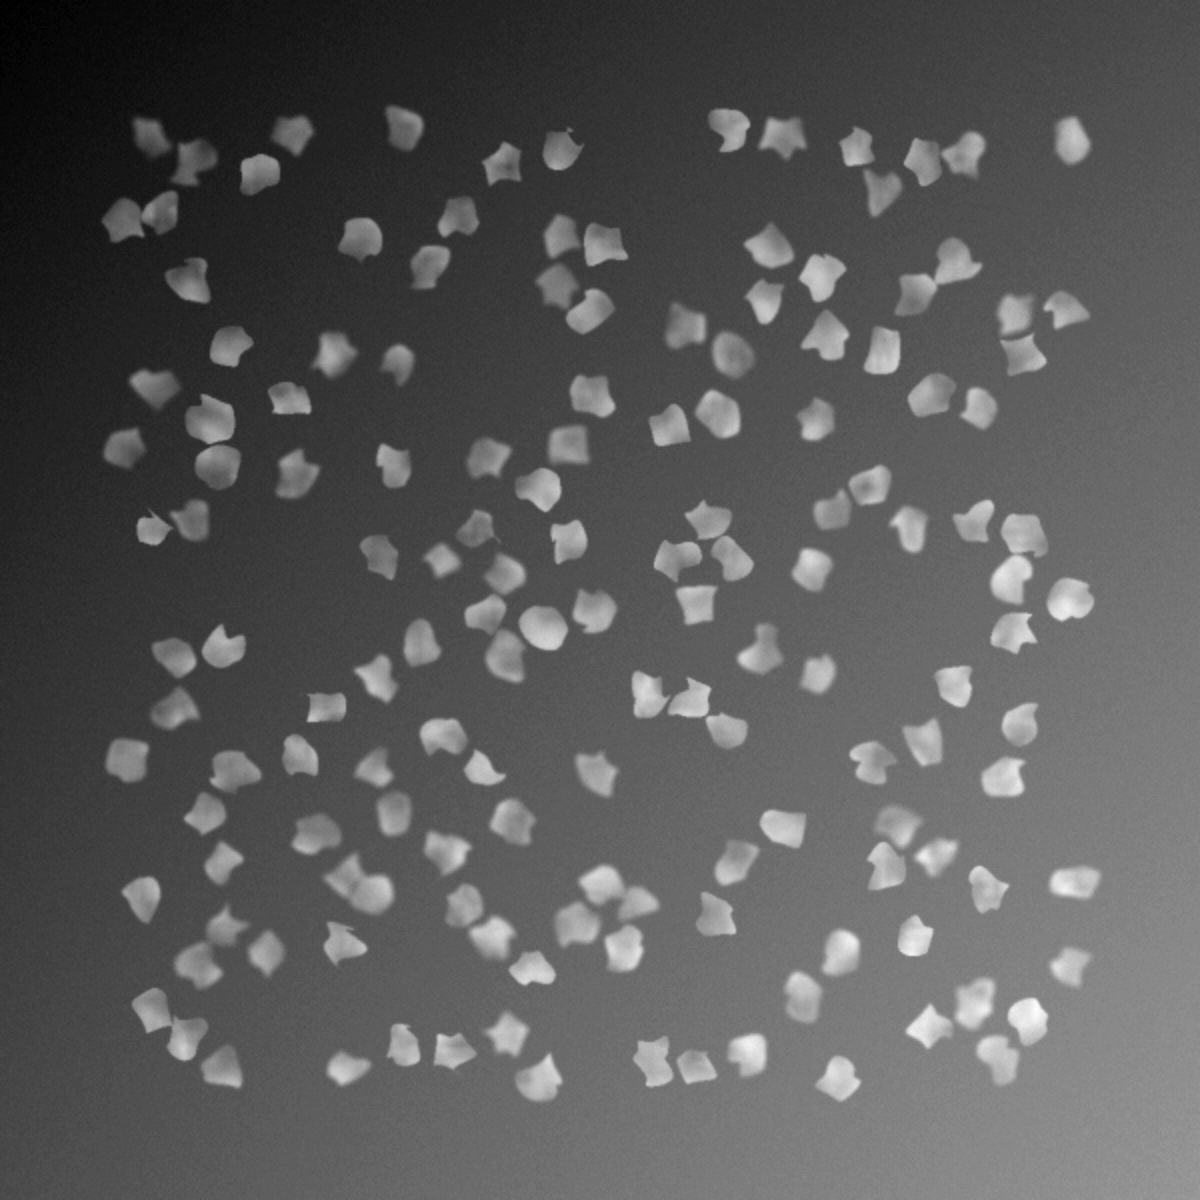
\includegraphics[width=0.3\linewidth]{cells.png}
    \caption{Useful figure}
    \label{fig:figurecell}
\end{figure}


\todo{Give an overview of the project.}

\todo{Answer questions from Website Chapter 1.3}

\todo{Motivate the project for medical approaches}

Figure \ref{fig:figurecell} shows ...

\section{Method}
\subsection{Thresholding and Illumination-Correction}
\todo{Answer questions about Chapter 1.4}

\subsection{Image Segmentation}
\todo{Answer questions about Chapter 2}

\todo{Provide the formulas for Specificity and Sensitivity.}
\begin{equation}
    Specificity =  \\
\end{equation}
\begin{equation} 
    Sensitivity = \\
\end{equation}

\subsection{Otsu's Method}
\todo{Cite \cite{Otsu}}

\todo{Answer questions about Chapter 3}
As mentioned in Section \ref{sec:introduction}. 


\subsection{Edge-detection}
\todo{Answer questions about Chapter 4}

\label{sec:edgedetection}

\subsection{Canny edge detection}
\todo{Answer questions about Chapter 5}

\begin{table}[]
    \centering
    \begin{tabular}{l|c|c|c|c|c}
        a & b & c & d & e & f \\
    \hline
        1 & 2 &0.2&0.3&0.4&0.5
    \end{tabular}
    \caption{In case you need a table.}
    \label{tab:my_label}
\end{table}

\newpage
\section{Conclusion}

\todo{Answer questions about Chapter 6}

% Literaturverzeichnis
\newpage
\bibliographystyle{apalike}
\bibliography{Bib/literatur}

\end{document}
  